\documentclass[]{article}
\usepackage{lmodern}
\usepackage{amssymb,amsmath}
\usepackage{ifxetex,ifluatex}
\usepackage{fixltx2e} % provides \textsubscript
\ifnum 0\ifxetex 1\fi\ifluatex 1\fi=0 % if pdftex
  \usepackage[T1]{fontenc}
  \usepackage[utf8]{inputenc}
\else % if luatex or xelatex
  \ifxetex
    \usepackage{mathspec}
  \else
    \usepackage{fontspec}
  \fi
  \defaultfontfeatures{Ligatures=TeX,Scale=MatchLowercase}
\fi
% use upquote if available, for straight quotes in verbatim environments
\IfFileExists{upquote.sty}{\usepackage{upquote}}{}
% use microtype if available
\IfFileExists{microtype.sty}{%
\usepackage{microtype}
\UseMicrotypeSet[protrusion]{basicmath} % disable protrusion for tt fonts
}{}
\usepackage[margin=1in]{geometry}
\usepackage{hyperref}
\hypersetup{unicode=true,
            pdftitle={RASP\_Report\_Prototype},
            pdfauthor={Army Research Institute and Northrop Grumman},
            pdfborder={0 0 0},
            breaklinks=true}
\urlstyle{same}  % don't use monospace font for urls
\usepackage{graphicx,grffile}
\makeatletter
\def\maxwidth{\ifdim\Gin@nat@width>\linewidth\linewidth\else\Gin@nat@width\fi}
\def\maxheight{\ifdim\Gin@nat@height>\textheight\textheight\else\Gin@nat@height\fi}
\makeatother
% Scale images if necessary, so that they will not overflow the page
% margins by default, and it is still possible to overwrite the defaults
% using explicit options in \includegraphics[width, height, ...]{}
\setkeys{Gin}{width=\maxwidth,height=\maxheight,keepaspectratio}
\IfFileExists{parskip.sty}{%
\usepackage{parskip}
}{% else
\setlength{\parindent}{0pt}
\setlength{\parskip}{6pt plus 2pt minus 1pt}
}
\setlength{\emergencystretch}{3em}  % prevent overfull lines
\providecommand{\tightlist}{%
  \setlength{\itemsep}{0pt}\setlength{\parskip}{0pt}}
\setcounter{secnumdepth}{0}
% Redefines (sub)paragraphs to behave more like sections
\ifx\paragraph\undefined\else
\let\oldparagraph\paragraph
\renewcommand{\paragraph}[1]{\oldparagraph{#1}\mbox{}}
\fi
\ifx\subparagraph\undefined\else
\let\oldsubparagraph\subparagraph
\renewcommand{\subparagraph}[1]{\oldsubparagraph{#1}\mbox{}}
\fi

%%% Use protect on footnotes to avoid problems with footnotes in titles
\let\rmarkdownfootnote\footnote%
\def\footnote{\protect\rmarkdownfootnote}

%%% Change title format to be more compact
\usepackage{titling}

% Create subtitle command for use in maketitle
\providecommand{\subtitle}[1]{
  \posttitle{
    \begin{center}\large#1\end{center}
    }
}

\setlength{\droptitle}{-2em}

  \title{RASP\_Report\_Prototype}
    \pretitle{\vspace{\droptitle}\centering\huge}
  \posttitle{\par}
    \author{Army Research Institute and Northrop Grumman}
    \preauthor{\centering\large\emph}
  \postauthor{\par}
      \predate{\centering\large\emph}
  \postdate{\par}
    \date{3/23/2020}


\begin{document}
\maketitle

\hypertarget{individual-report-for-a1000}{%
\subsection{Individual Report for:
A1000}\label{individual-report-for-a1000}}

\hypertarget{personality}{%
\subsubsection{Personality}\label{personality}}

\hypertarget{personality-this-graph-displays-results-from-the-jpi-r-personality-test-in-green-bars.}{%
\subparagraph{\texorpdfstring{Personality: This graph displays results
from the JPI-R Personality Test in \textbf{green
bars}.}{Personality: This graph displays results from the JPI-R Personality Test in green bars.}}\label{personality-this-graph-displays-results-from-the-jpi-r-personality-test-in-green-bars.}}

The \textbf{RED dots} represent the average of all Ranger Candidates.
The \textbf{BLUE dots} represent the measures used to determine the
cyber fit score and the objective value for the measure.

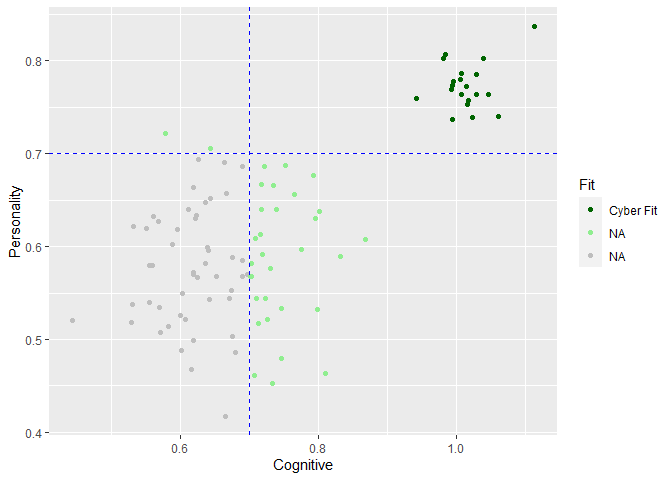
\includegraphics{RASP_MarkdownReport_files/figure-latex/unnamed-chunk-1-1.pdf}

\hypertarget{cognitive}{%
\subsubsection{Cognitive}\label{cognitive}}

\hypertarget{cognitive-this-graph-displays-results-from-the-mab-ii-cognitive-test-in-green-bars.}{%
\subparagraph{\texorpdfstring{Cognitive: This graph displays results
from the MAB II Cognitive Test in \textbf{green
bars}.}{Cognitive: This graph displays results from the MAB II Cognitive Test in green bars.}}\label{cognitive-this-graph-displays-results-from-the-mab-ii-cognitive-test-in-green-bars.}}

The \textbf{RED dots} represent the average of all Ranger Candidates.
The \textbf{BLUE dots} represent the measures used to determine the
cyber fit score and the objective value for the measure.

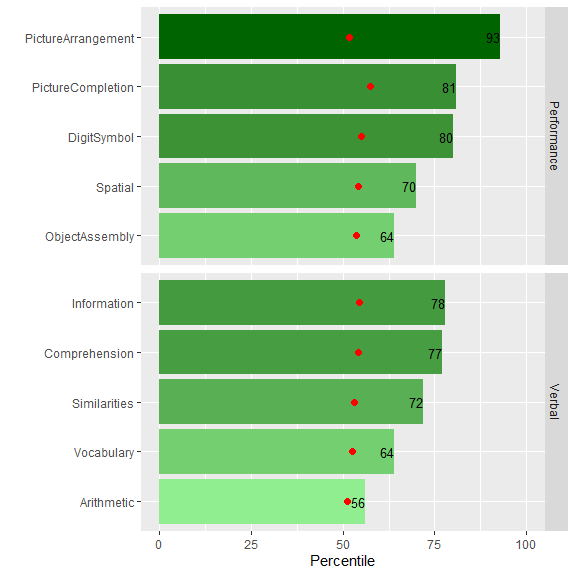
\includegraphics{RASP_MarkdownReport_files/figure-latex/unnamed-chunk-2-1.pdf}

\hypertarget{results-from-the-cyber-fit-model-for-a1000.}{%
\subsection{Results from the Cyber Fit model for
A1000.}\label{results-from-the-cyber-fit-model-for-a1000.}}

Cyber Fit Scores are weighted scores based on multiple measures within
each category. The maximum score is 1.0. The dashed blue line represents
a threshold cyber fit score, above which suggests a good fit.

The \textbf{GREEN dots} represents the Cyber Fit Scores for
\textbf{A1000} in each Category. The total RASP candidate distribution
is displayed by the boxplot. This individual's Cyber Fit Score ranks
\textbf{6} of \textbf{99} in the RASP data repository.

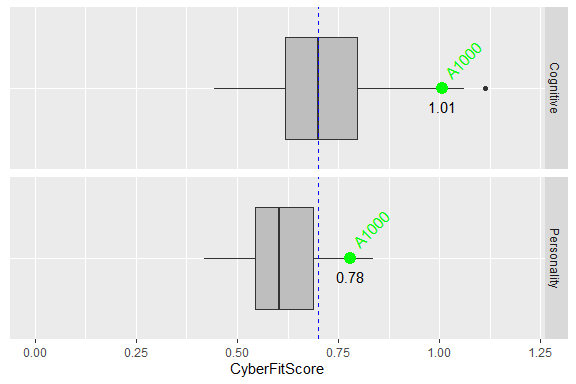
\includegraphics{RASP_MarkdownReport_files/figure-latex/unnamed-chunk-3-1.pdf}

\hypertarget{section}{%
\subsection{}\label{section}}


\includegraphics[width=1.5625in,height=\textheight]{RangerInsignia.jpg}


\end{document}
